\documentclass{article}

\textwidth=6.5in
\textheight=8.5in
\voffset=-54pt
\oddsidemargin=0in
\evensidemargin=0in
\setlength{\parskip}{8pt}
\setlength{\parindent}{0pt}

\usepackage[normalem]{ulem}

\usepackage{amsmath, amssymb}
\usepackage{ifthen}

\usepackage[inline]{enumitem}
\setlist{topsep=0pt, parsep=8pt}

\usepackage[rgb,table]{xcolor}\convertcolorsUfalse
\usepackage{graphicx}

% change hyperref options
\PassOptionsToPackage{hyphens}{url}
\usepackage[bookmarks,colorlinks,linkcolor=black,citecolor=blue,pdfstartview=FitH,urlcolor=blue]{hyperref}
\hypersetup{pdfpagemode=UseNone}
\usepackage{bookmark}

\usepackage{graphicx}
\usepackage{multicol}
\usepackage{framed}
\usepackage{array}

\usepackage{icomma}

\usepackage{marginnote}
\usepackage[colorinlistoftodos]{todonotes}
\renewcommand{\marginpar}{\marginnote}

\usepackage{soul}

\usepackage{pgfplots}
\pgfplotsset{compat=1.18}  
\pgfplotscreateplotcyclelist{mycolor}{black, blue, red, green!70!black, magenta, purple, cyan, orange }  
\pgfplotsset{
  disabledatascaling,
  cycle list=tikzcolor, 
  axis lines=middle,
  every axis plot/.style={no marks, thick},
  every axis/.style={
    enlarge x limits=false,
    enlarge y limits=auto,
    xlabel style={at={(current axis.right of origin)},anchor=west},
    ylabel style={at={(current axis.above origin)},anchor=south},
    % extra x and y ticks for asymptotes
    extra x tick style={grid=major, grid style={dashed,black}},
    extra y tick style={grid=major, grid style={dashed,black}},
    /pgf/number format/1000 sep={},
  },    
  tick label style = {font=\footnotesize, fill=\currentbgcolor, inner sep=0pt},    
  xticklabel shift=1pt,    
  scaled ticks=false,
  scaled y ticks=false,
  unbounded coords=jump,
  samples=101,
  minor tick length=0,
  scatter/classes={
    open={mark=*,draw=black,fill=white, mark size=2, thin},
    closed={mark=*,draw=black,fill=black, mark size=2, thin}
  },
  width=3in,
}
\pgfplotsset{open/.style={only marks, mark=*, fill=white, thin, mark size=2}}
\pgfplotsset{closed/.style={only marks, mark=*, draw=black, fill=black,
    thin, mark size=2}}
\pgfplotsset{labeled/.style={nodes near coords, only marks, mark=*, draw=black, fill=black, thin, mark size=2, point meta=explicit symbolic}}

\usepackage{tikz}
\usetikzlibrary{
  matrix,%
  % enables the snake paths
  decorations.pathmorphing,%
  % enables bigger arrows
  decorations.markings,%
  decorations.pathreplacing,%
  decorations.text,%
  calc,%
  patterns,%
  shapes.geometric,%
  arrows,
  decorations.shapes,
  positioning,
  plotmarks,
  intersections
}
\tikzset{>=latex} % sets default arrow type in tikz
\tikzset{font=\normalsize}
\tikzset{mark size=1.5pt, mark options=thin}
\tikzset{pin distance=4pt,
  every pin edge/.style={<-, thin, shorten <= -2pt}}

\interfootnotelinepenalty=10000
\renewcommand{\thefootnote}{(\arabic{footnote})}

\usepackage{multirow, bigdelim}

% change to \usepackage[sols]{handout} to see solutions
\usepackage[]{handout}
\renewcommand{\workshopnote}{CA Notes.}    

\newcommand\iscurrentenumi[1]{%
  \ifthenelse{\equal{#1}{\theenumi}}{}{#1}}
\setenumerate[1]{ref=\#\arabic*}
\setenumerate[2]{ref=\protect\iscurrentenumi{\theenumi}(\alph*)}
\newcommand\enumiiprefix[2]{%
  \ifthenelse{{\equal{#1}{\theenumi}}\AND{\equal{#2}{(\alph{enumii})}}}{}{}%
  \ifthenelse{{\equal{#1}{\theenumi}}\AND{\NOT{\equal{#2}{(\alph{enumii})}}}}{#2}{}%
  \ifthenelse{\equal{#1}{\theenumi}}{}{#1#2}%
}
\setenumerate[3]{ref=\protect\enumiiprefix{\theenumi}{(\alph{enumii})}\roman*}

\makeatletter

% underline links               
\let\@href=\href
\renewcommand{\href}[2]{\@href{#1}{\ul{#2}}}

\newcommand\calculator{
  
\begin{tikzpicture}[x=0.15ex, y=0.15ex, baseline=1.5pt]
    \begin{scope}[thick]
      \draw (0, 0) -- (10, 0) -- (10, 14) -- (0, 14) -- cycle;
      \foreach \x in {10/3, 20/3}
      {
        \draw (\x, 0) -- (\x, 10);
      }
      \foreach \y in {10/3, 20/3, 10}
      {
        \draw (0, \y) -- (10, \y);
      }
    \end{scope}
  \end{tikzpicture}
}
\newcommand{\calcitem}{\refstepcounter{enum\romannumeral\@enumdepth}%
\item[\calculator \csname labelenum\romannumeral\@enumdepth\endcsname]}

\makeatother

\definecolor{purple}{rgb}{0.5,0,1.0}

\newcommand{\doedfinity}[2][\newpage]{
  \begin{problem}[#1]
    Do the Edfinity assignment ``Problem Set #2''.

    We encourage you to write down any scratch work here, as well as
    things you want your future self to remember. Nothing you write
    here will be graded; it's just for you!
  \end{problem}
}

\newcommand{\psrnewpage}{\newpage}
\newcommand{\psreflection}[2][]{

  \ifthenelse{\not\equal{#1}{nocite}}{
    \begin{enumerate}[resume]
    \item
      \begin{problem}[1in]
        Please cite any help you got on this problem set:
        \begin{itemize}[nosep]
        \item If you worked with other students, please list their names here.
        \item If you used resources other than those on our Canvas site, please list them here.
        \end{itemize}
      \end{problem}

    \end{enumerate}
  }

  \probonly{%
    #2

    \psrnewpage

    \emph{Reflection space.} It's a good habit to take a few minutes at the end of each pset to reflect on what you learned and jot down notes to your future self. Here are a few reflection questions to get you started. Nothing you write here will be graded; it's just for you!
    \begin{itemize}
    \item Take a few minutes to look back at the problems. How could you explain to someone else how to do each problem? What was your strategy, and how did you know to use that strategy? If there are problems where you don't feel able to answer this, write down which ones they are. Come back to them in a few days when we post the homework solutions!

      \vspace{1.5in}

    \item Take a look back at the learning objectives on today's worksheet; how are you feeling about each one? If there are ones you know you need more practice with, write those down here.

      \vspace{1.5in}

    \item What did you find most challenging about this material? Do you have any lingering questions about it? If so, write them down here so you don't forget them. At some point, stop by office hours or MQC to ask!

      \vfill
    \end{itemize}      
  }
}

\usepackage{fancyhdr}
\lhead{\textcolor{white}{This content is protected and may not be shared, uploaded, or distributed.}}
\rhead{}
\rfoot{\vspace*{\fill}\footnotesize\textcopyright{} \emph{Harvard Math Ma}}
\renewcommand{\headrulewidth}{0pt}
\pagestyle{fancy}
\begin{document}

\begin{center}
  \large\textsc{Problem Set 32 - Derivatives of Logarithmic and Exponential Functions}
\end{center}

\begin{enumerate}
\item  \note{
    \begin{itemize}[nosep]
    \item Some derivatives of logs and exponentials that don't require rewriting with log / exp rules
    \item Find critical points of something like $x^5 \ln x$
    \item Rewrite some exponential functions as $C \cdot b^x$ and $C e^{kx}$, and differentiate them.
    \item Given a graph of $f$, match $3 f(x) + 2$, $f'(x)$, and $f^{-1}(x)$ with graphs.
    \end{itemize}
  }

  \doedfinity{32}

\item  In each part, you're given $y$ in terms of $x$. Rewrite $y$ so that you can differentiate it, and then find $y'$. You need not simplify $y'$, but be sure to show your work when you rewrite $y$.

  \begin{enumerate}
  \item

    \begin{grading}
      2.5 points:
      \begin{itemize}[nosep]
      \item 1.5 for simplifying $y$. A possible breakdown is:
        \begin{itemize}[nosep]
        \item 0.5 for knowing $\ln \left( \dfrac{\sqrt[4]{x^3}}{2} \right) = \ln \left( \sqrt[4]{x^3} \right) - \ln 2$
        \item 0.5 for $\ln \left( \sqrt[4]{x^3} \right) = \dfrac{3}{4} \ln x$
        \item 0.5 for keeping the $e$ in the right place when simplifying $y$
        \end{itemize}
      \item 1 for differentiating their simplified $y$ correctly
      \end{itemize}
    \end{grading}

    \begin{problem}[\vfill]
      $\displaystyle y = \frac{\ln \left( \dfrac{\sqrt[4]{x^3}}{2} \right)}{e}$
    \end{problem}

    \begin{solution}
        \begin{align*}
          y &= \frac{\ln \left( \dfrac{\sqrt[4]{x^3}}{2} \right)}{e} \\
          &= \frac{1}{e} (\ln \sqrt[4]{x^3} - \ln 2) \\
          &= \frac{1}{e} \left(\frac{3}{4} \ln x - \ln 2\right) \\
          y' &= \frac{1}{e} \left(\frac{3}{4x}\right)\\
          &= \boxed{\frac{3}{4ex}}
        \end{align*}
    \end{solution}

  \item

    \begin{grading}
      3 points:
      \begin{itemize}[nosep]
      \item 1.5 for simplifying $y$. A possible breakdown is:
        \begin{itemize}[nosep]
        \item 0.5 for $\ln(ex^2) = \ln(e) + \ln(x^2)$
        \item 0.5 for $\ln(x^2) = 2 \ln x$
        \item 0.5 for keeping track of what's multiplied by $7^x$
        \end{itemize}
      \item 1.5 for differentiating their simplified $y'$ correctly. If they don't use Product Rule, they can get at most $0.5$. 
      \end{itemize}
    \end{grading}

    \begin{problem}[\vfill]
      $y = 7^x \ln (e x^2)$
    \end{problem}

    \begin{solution}
      \begin{align*}
        y &= 7^x \ln(ex^2) \\
        &= 7^x (\ln(e) + \ln(x^2)) \\
        &= 7^x (\ln(e) + 2\ln(x)) \\
        y' &= 7^x \ln(7)(\ln(e) + 2\ln(x)) +
        7^x \left(\frac{2}{x}\right) \\
        &= 7^x\left(\ln(7)\ln(e) + 2\ln(7)\ln(x) + \frac{2}{x}\right)
      \end{align*}
    \end{solution}

  \end{enumerate}

\item %({\it 14.1.12}) Use a tangent line approximation to approximate: (a) $\ln(0.9)$, and (b) $\ln(1.1)$.  ({\it Hint: what is a ``nice" number nearby?})

  \begin{enumerate}
  \item

    \begin{grading}
      5 points:
      \begin{itemize}[nosep]
      \item 1 for knowing to find the tangent line at $x = 1$
      \item 2 for correctly finding the equation of the line
      \item 1 for correctly using the line to estimate the given values
      \item 1 for a picture showing $\ln x$ and the tangent line at $x = 1$ 
      \end{itemize} 
    \end{grading} 

    \begin{problem}[\nstretch{2}]
      Use a tangent line approximation to approximate $\ln(0.9)$ and $\ln(1.1)$. Sketch a picture illustrating your approximations. 
    \end{problem}

    \begin{solution} 
      We will use the tangent line at $x=1$ to  the curve $f(x) = \ln(x)$ to make our approximations. 
      $$f'(x)= \frac{1}{x}$$  
      $$f'(1) = 1 $$ 
      Using point slope: 
      $$y-0 = 1(x-1)$$ 
      so 
      $$\ln(x) \approx x- 1 \text{ for $x$ near 1} $$ 
      \begin{center} 
          $\ln(.9) \approx .9-1 =-.1$ and $\ln(1.1) \approx1.1-1=.1$.
      \end{center} 

      \begin{center}
        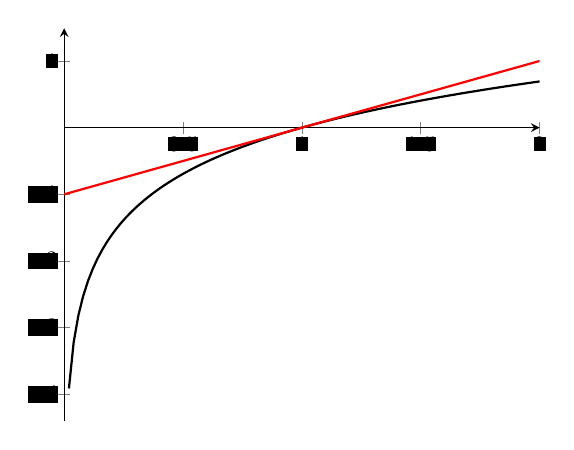
\begin{tikzpicture}
          \begin{axis}
            \addplot[domain=0:2] {ln(x)};
            \addplot[red,domain=0:2] {x-1};
          \end{axis}
        \end{tikzpicture}
      \end{center}
    \end{solution} 

  \item

    \begin{grading}
      1 point
    \end{grading}

    \begin{problem}[1in]
      Based on the picture, are your approximations overestimates or underestimates? Explain briefly. 
    \end{problem}

    \begin{solution}
      Based on the picture, our approximations
      are overestimates, because the tangent
      line to $y=\ln x$ at $x=1$
      is above the graph.
    \end{solution}

  \end{enumerate}

\item \label{intro-to-exp-log-equations}

  Solve the following equations for the indicated variable. The first step in each is to translate the given equation: if it involves a log, translate it into an exponential equation; if it involves an exponential, translate it into a logarithmic equation. (a) is done for you as an example.

  \begin{grading}
    2 points per part: 1 for correctly translating the given equation into a log/exponential equation, 1 for solving after that. 
  \end{grading}

  \begin{enumerate}
  \item

    \begin{grading}
      Nothing to grade here
    \end{grading}

    \begin{problem}
      Solve $3^{4t + 1} = 5$ for $t$. 
    \end{problem}

    \textbf{Solution.} The equation $3^{4t + 1} = 5$ says ``$4t + 1$ is the power we raise 3 to in order to get 5.'' We can rewrite this as
    \begin{align*}
      4t + 1 &= \log_3 5 \\
      \intertext{From here, we can subtract 1 from both sides and then divide by 4:}
      4t &= \log_3 5 - 1 \\
      t &= \boxed{\frac{\log_3 5 - 1}{4}} 
    \end{align*}

  \item

    \begin{problem}[\vfill]
      Solve $\log_2 (5w + 4) = \dfrac{1}{2}$ for $w$.
    \end{problem}

    \begin{solution}
      This equation says ``$\frac{1}{2}$ is the power we raise $2$ to in order to get 
      $(5w+4)$. We can rewrite this as
      \begin{align*}
        5w+4 &= 2^{1/2} \\
        \intertext{From here, we can solve for $w$.}
        5w + 4 &= \sqrt{2} \\
        5w &= \sqrt{2}-4 \\
        w &= \boxed{\frac{\sqrt{2}-4}{5}}.
      \end{align*}
    \end{solution}

  \item
    \begin{problem}[\vfill\newpage]
      Solve $e^{2 - s / 4} = 7$ for $s$.
    \end{problem}

    \begin{solution}
      This equation says ``$2-\frac{s}{4}$ is the
      power we raise $e$ to in order to get $7$.''
      We can rewrite this in logarithmic form as
      \begin{align*}
        \ln(7) &= 2-\frac{s}{4} \\
        \intertext{Now we can solve for $s$.}
        \ln(7) + \frac{s}{4} &= 2 \\
        \frac{s}{4} &= 2-\ln(7) \\
        s &= \boxed{4(2-\ln7)}
      \end{align*}
    \end{solution}

  \end{enumerate}

\item %({\it 14.1.14})

  Let $f(x) = \ln(x) -x$

  \begin{enumerate}
  \item

    \begin{grading}
      0.5 points
    \end{grading}

    \begin{problem}[0.5in]
      What's the domain of $f$? 
    \end{problem}

    \begin{solution}
      We can't take the logarithm of a negative
      number, so the domain is $\boxed{(0, \infty)}$.
    \end{solution}

  \item

    \begin{grading}
      3 points: 0.5 for finding $f'$ correctly, 0.5 for solving for where $f' = 0$, 2 points for using a correct method to classify (either First or Second Derivative Test). If they classify but don't show any work, deduct 1.5. 
    \end{grading}

    \begin{problem}[\vfill]
      Find and classify all the critical points of $f$. (Remember that the critical points must be in the domain of $f$.) Please make it clear to your reader how you're classifying the critical points. 
    \end{problem}

    \begin{solution}

       $f'(x) = \frac{1}{x} -1$. To find the critical points we look for where $f'(x) = 0$ and where $f'(x)$ does not exist on the domain. 
        $$f'(x) = \frac{1}{x} - 1 = 0$$ 
        $$ \frac{1}{x} = 1$$ 
        $$x=1$$ 

        We can use the Second Derivative Test to classify this critical point.

        \begin{align*}
          f''(x) &= -\frac{1}{x^2} \\
          f''(1) &= -1
        \end{align*}
        Since $f''(1)$ is negative, \fbox{$x=1$ is a
        local maximum}.
    \end{solution} 

  \item

    \begin{grading}
      2 points
    \end{grading}

    \begin{problem}[\nstretch{0.75}]
      Where is $f$ concave up? Where is $f$ concave down? 
    \end{problem}

    \begin{solution} 
      The second derivative will tell us about the concavity. $$ f''(x) = -\frac{1}{x^2}$$ is negative everywhere. This means that the function is \fbox{concave down everywhere}.
    \end{solution} 

  \item

    \begin{grading}
      1 point
    \end{grading}

    \begin{problem}[1.5in]
      What is $\displaystyle \lim_{x \to 0^+} f(x)$? Explain briefly. 
    \end{problem}

    \begin{solution}
      As $x$ approaches $0$ from the right,
      $\ln(x)$ goes to $-\infty$ and $x$ approaches
      $0$, so $\ln(x) -x$ goes to $\boxed{-\infty}$.
    \end{solution}

  \item

    \begin{grading}
      4 points:
      \begin{itemize}[nosep]
      \item 1 for being consistent with the domain they found in (a)
      \item 1 for being consistent with the critical points they found in (b)
      \item 1 for being consistent with the concavity they found in (c)
      \item 1 for being consistent with the limit they found in (d)
      \end{itemize}
    \end{grading}

    \begin{problem}[\vfill\newpage]
      Without using technology, sketch a graph of $f(x) = \ln (x) - x$, clearly labeling any critical points and inflection points with their simplified exact coordinates (both $x$- and $y$-coordinates).
    \end{problem}

    \begin{solution}
      There is no inflection point. The critical point is $(1, f(1)) = (1, -1)$. 
      \begin{center}
        \begin{tikzpicture}
          \begin{axis}[ymax=1, xtick={1}, ytick={-1}]
            \addplot+[domain=0:4]{ln(x) -x}; %
            \addplot+[closed] coordinates { (1, -1) } node[above]{$(1, -1)$}; 
          \end{axis}
        \end{tikzpicture}
      \end{center}
    \end{solution}

  \end{enumerate} 

\item  

  The U.S. Fish and Wildlife Service has tracked the sea otter population in Washington State for many years. 
  According to \href{https://wdfw.wa.gov/sites/default/files/publications/00314/wdfw00314.pdf}{Washington State's 2004 sea otter recovery plan}, in July 1993, there were about 300 sea otters in Washington; in July 1999, there were about 600. 

  Let's assume the sea otter population is an exponential function of time. 

  \begin{enumerate}
  \item

    \begin{grading}
      3 points:
      \begin{itemize}[nosep]
      \item 1 for correctly interpreting the given information (for example, by recognizing that, if $P(t)$ is the population at time $t$, we know $P(3) = 300$ and $P(9) = 600$)
      \item 1 for correctly finding that, if $P(t) = C \cdot b^t$, then $b = 2^{1/6}$
      \item 1 for correctly finding that $C = \dfrac{300}{\sqrt{2}}$
      \end{itemize}
    \end{grading}

    \begin{problem}[\stretch{2}]
      Write a formula for the sea otter population $t$ years after July 1990 (assuming the population is an exponential function of time). 
    \end{problem}

    \begin{solution}
      If $P(t)$ is the population $t$ years 
      after 1990, then $P(3)=300$ and $P(9)=600$.
      Let's say $P(t)= C\cdot b^t$. Then
      \begin{align*}
          Cb^{3} &= 300 \\
          Cb^{9} &= 600
      \end{align*}
      Dividing the second equation by the 
      first equation gives us $b^6 = 2$, so
      $b = 2^{1/6}$. This means that 
      $C(2^{1/6})^3 = \sqrt{2}C = 300$, so $C=\frac{300}{\sqrt{2}}$. 
      Thus, $P(t) = \boxed{\frac{300}{\sqrt{2}} 2^{t/6}}$.
    \end{solution}

  \calcitem

    \begin{workshop}
      If students are having trouble with this, see if they can get the equation to look like something in \ref{intro-to-exp-log-equations}. 
    \end{workshop}

    \begin{grading}
      \begin{itemize}[nosep]
      \item 0.5 for recognizing we want to solve $P(t) = 900$
      \item 2 points for solving correctly for $t$
      \item 1 point for correctly translating this into a year. (If they say 2002 instead of 2003, deduct 0.25.) 
      \end{itemize}
    \end{grading}

    \begin{problem}[\vfill\newpage]
      According to this model, when did the otter population reach 900? Give an exact answer, and then use \href{https://www.wolframalpha.com/}{WolframAlpha} to figure out what year this corresponds to. (In WolframAlpha, you can get the decimal value of an expression like $3 \log_5(7)$ by typing \verb!3 log_5(7)!.)
    \end{problem}

    \begin{solution}
      We want to solve for $t$ in $\frac{300}{\sqrt{2}} 2^{t/6} = 900$.
      \begin{align*}
          \frac{300}{\sqrt{2}} 2^{t/6} &= 900 \\
          2^{t/6} &= 3\sqrt{2} \\
          \tfrac{1}{6}t &= \log_2{3\sqrt{2}} \\
          \tfrac{1}{6}t &= \log_2{3} + \tfrac{1}{2}\\
          t &= 6\log_2{3} + 3 \\
          &\approx 12.51
      \end{align*}
      This means that the otter population will
      reach 900 in \fbox{2003}.
    \end{solution}

  \item

    \begin{grading}
      \begin{itemize}[nosep]
      \item 1 for recognizing they want $P'(3)$
      \item 1 for calculating $P'(t)$ correctly
      \item 1 for calculating and simplifying $P'(3)$ correctly. (It's okay if they leave it as $300 \ln \left( 2^{1/6} \right)$, but they shouldn't have $\sqrt{2}$ left.)
      \item 1 for units
      \end{itemize}
    \end{grading}

    \begin{problem}[\vfill]
      According to this model, how quickly was the otter population changing in July 1993? Give an instantaneous rate of change; please simplify your answer, and include units.
    \end{problem}

    \begin{solution}
      We should find $P'(3)$ by first finding $P'(t)$. We can rewrite $P(t)$ as
      \begin{align*}
        P(t)&=\frac{300}{\sqrt{2}} 2^{t/6}\\ &= 
        \frac{300}{\sqrt{2}} (2^{1/6})^t
        \intertext{Now we can take the derivative.}
        P'(t) &= \frac{300}{\sqrt{2}} (\ln 2^{1/6})
        (2^{1/6})^t \\
        &= \frac{300}{\sqrt{2}}(\tfrac{1}{6}\ln 2)(2^{t/6}) \\
        &= \frac{50\ln 2}{\sqrt{2}}2^{t/6}
        \intertext{So $P'(3)$ is}
        P'(3) &= \frac{50\ln 2}{\sqrt{2}} 2^{1/2} \\
        &= \boxed{50 \ln 2\text{ otters per year}}
      \end{align*}
    \end{solution}

  \end{enumerate}

\item 
\begin{problem}
    Next class, we're going to combine our knowledge of derivatives we've learned til this point to differentiate compositions of many types of functions using the Chain Rule. To refresh your memory, compute the derivatives of the following functions (you do not need to simplify):
\end{problem}
\begin{enumerate}
    \item 
    \begin{problem}[\vfill]
    Find $f'(x)$ if $\displaystyle f(x) = \sqrt{3x^2-x}$\\
    \end{problem}
    \begin{solution}
        $\displaystyle f'(x) = \frac{1}{2}(3x^2-2)^{-1/2}\cdot (6x)$
    \end{solution}

    \item 
    \begin{problem}[\vfill]
        Find $f'(x)$ if $\displaystyle f(x) = \frac{3-x}{(x^2+6x)^2}$\\
        
    \end{problem}
\begin{solution}
        $\displaystyle f(x) = \frac{3-x}{(x^2+6x)^2}=(3-x)(x^2+6x)^{-2}$\\
        Differentiating, we use the product rule and the chain rule in order to find the derivative of the second term.\\
        $f'(x)=(-1)(x^2+6x)^-2+(3-x)(-2(x^2+6x)^{-3}(2x+6))$
    \end{solution}

    \item 
    \begin{problem}[\vfill]
        Compute $\frac{d}{dx} [f(x^2)]^3$.\\
    \end{problem}

    \begin{solution}
        $\frac{d}{dx} [f(x^2)]^3=3[f(x^2)]^2\cdot f'(x^2)\cdot (2x)$
    \end{solution}
    \end{enumerate}
\end{enumerate}

\psreflection{For next class, read \S 13.3.}
\end{document}
